\documentclass[a4paper, 12pt, titlepage]{article}
\usepackage[utf8]{inputenc}
\usepackage{geometry}
\usepackage{polski}
\usepackage{graphicx}
\usepackage{float}
\usepackage{etoolbox,refcount}
\usepackage{multicol}
\usepackage{fancyhdr}
\pagestyle{fancy}
\title{Badanie właściwości metrologicznych toru pomiarowego z modulacją AM przeznaczonego do współpracy z czujnikami wielkości nieelektrycznych}
\author{\textbf{Adrian Jałoszewski}, Tomasz Kotowski, Monika Ścisło}
\date{10 października 2016, poniedziałek, $9^{\underline{30}}$}
\newgeometry{left=2.5cm, right=2.5cm, bottom=2.5cm, top=2.5cm}

\begin{document}
	\maketitle
	\tableofcontents
	\newpage
	\section{Cel ćwiczenia}
	Celem ćwiczenia było zapoznanie się z pomiarem wielkości nieelektrycznej jaką jest przesunięcie przy pomocy przyrządów mierzących wielkości elektryczne.
	\section{Wykaz aparatury}
	\begin{enumerate}
		\item Układ pomiarowy -- tor z modulacją amplitudy
		\item Multimetr HP34401A lub HP34410A (łącznie dwie sztuki)
		\item Oscyloskop dwukanałowy Tektronix TDS1012B
		\item Czujnik transformatorowy PTx20 firmy Peltron zintegrowany mechanicznie ze śrubą mikrommetryczną
	\end{enumerate}
	\section{Wykonanie ćwiczenia}
		Ćwiczenie było wykonane dla obydwu podpunktów punktu pierwszego oraz dla punktu trzeciego. Punkt drugi został pominięty w wykonaniu pomiarów ze względu na to, że dane potrzebne do jego realizacji zostały pobrane w trakcie wykonania pozostałych dwóch punktów.
		\subsection{Badanie właściwości metrologicznych transformatorowego czujnika LVDT drogi}
			Pomiary mają na celu wyznaczenie charakterystyki czujnika oraz obserwację przebiegów czasowych w torze przetwarzania wzmacniacza z modulacją AM. Badany tor pomiarowy jest złożony z transformatorowego czujnika LVDT zbudowanego na bazie układu scalonego NE5521, który zawiera oscylator generujący sygnał zasilającyczujnik oraz elementy przetwarzania: 
			\begin{itemize}
				\item[--] wzmacniacz zmiennoprądowy
				\item[--] demodulator fazoczuły
				\item[--] filtr dolnopasmowy
			\end{itemize}
			\subsubsection{Wyznaczenie charakterystyki statycznej czujnika LVDT}
				Poniższy schemat przedstawia połączenia w układzie dla punktu pierwszego ćwiczenia. Zawarte na nim jest poprawne podłączenie multimetrów, z których mierzy wartość napięcia referencyjnego, a drugi wartość skuteczną napięcia. %todo nazwać napięcia
				\begin{figure}[H]
					\centering
					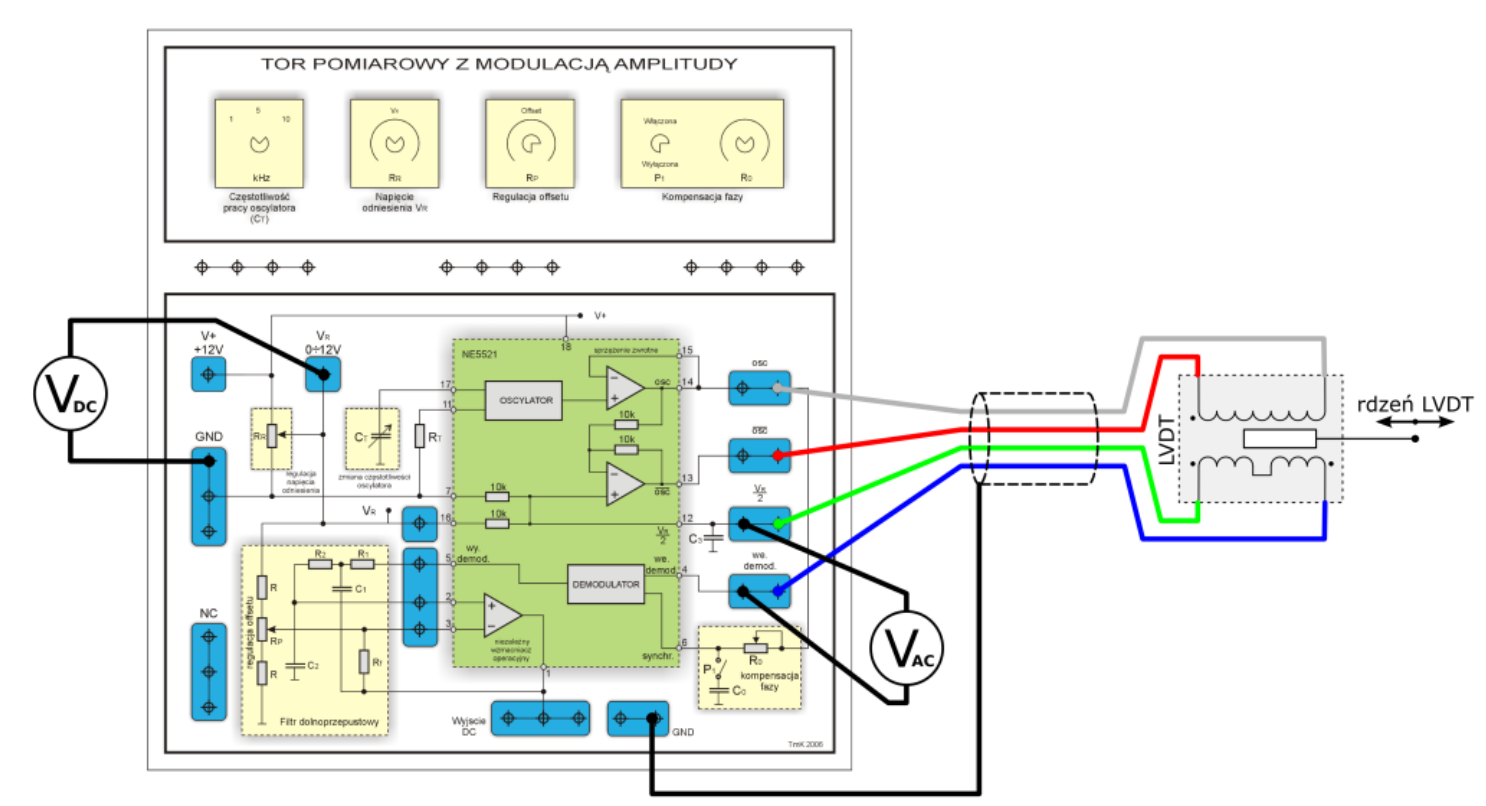
\includegraphics[width=0.8\textwidth]{./img/tor_pierwsze.png}
					\caption{\small{Schemat połączeń przy współpracy toru pomiarowego z czujnikiem LVDT}}
				\end{figure} \noindent
				Aby wyznaczyć charakterystykę statyczną czujnika LVDT rozpoczęliśmy od ustawienia poprawnego napięcia referencyjnego tak aby jego wartość była jak najbliższa $10\,\mathrm{V}$. Strojenia dokonaliśmy przy pomocy potencjometru ${R_R}$.
				\newline \newline
				Następnie przystąpiliśmy do wyznaczenia zera konstrukcyjnego czujnika -- szukaliśmy takiego położenia dla którego wystąpi minimalne wskazanie dla mierzonego napięcia przemiennego. Minimum te znaleźliśmy dla wartości 62,2 mm.
				\newline \newline
				Pomiarów dokonaliśmy więcej niż było wymagane przez ćwiczenie. Pomiary były wykonywane co 0,5 mm w zakresie od 50,5 mm do 72 mm. Dodatkowy pomiar został wykonany dla zera konstrukcyjnego czujnika.
				\begin{figure}[H]
					\centering
					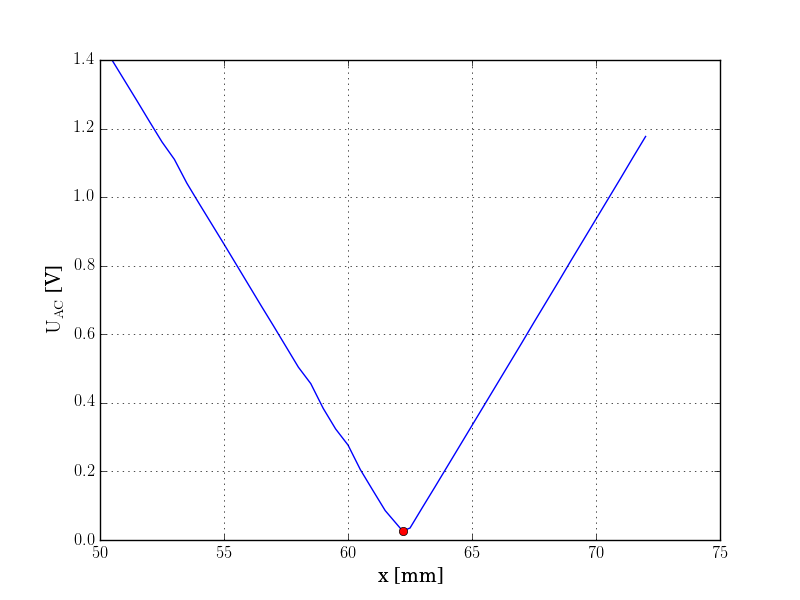
\includegraphics[width=0.75\textwidth]{./img/Uac_od_x.png}
					\caption{\small{Zależność wartości skutecznej napięcia od położenia rdzenia}}
				\end{figure} \noindent
				Do wyznaczenia błędu bezwzględnego potrzebna jest charakterystyka czujnika, która dla wartości poniżej zera konstrukcyjnego przyjmuje wartości ujemne. Po dokonaniu tej modyfikacji na zestawie danych mogliśmy wyznaczyć zależność błędu bezwzględnego danego wzorem $\Delta_U = U_{pomiar} - U_{oblicz}$. Gdzie $U_{oblicz}$ uzyskaliśmy dzięki regresji liniowej. Prosta najlepiej dopasowana do charakterystyki jest zadana wzorem: $y = 0.1198 \cdot x -7.455$
				\begin{figure}[H]
					\centering
					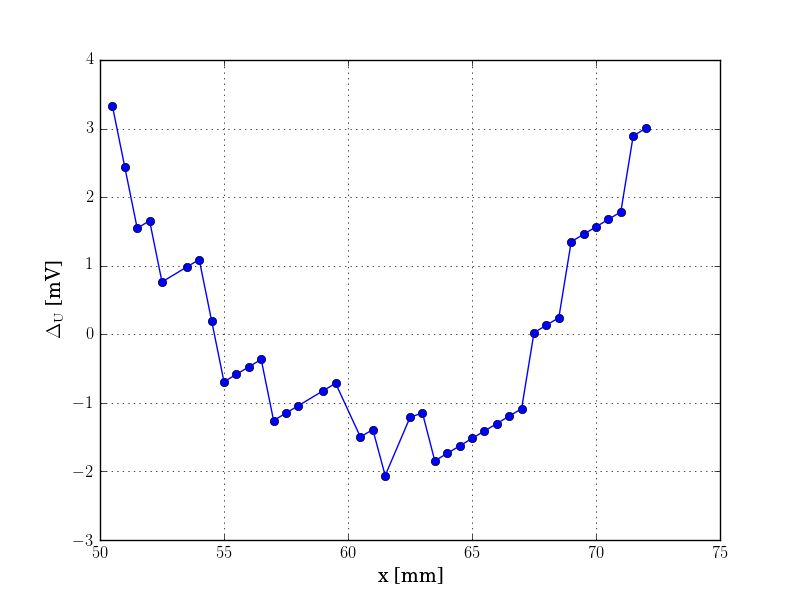
\includegraphics[width=0.8\textwidth]{./img/Uac_blad.png}
					\caption{\small{Zależność błędu bezwzględnego od położenia rdzenia}}
				\end{figure} \noindent
				Na podstawie tych danych wyznaczyliśmy błąd nieliniowości $\delta_{U_{max}} = 0,981\cdot10^{-3}$ zadany wzorem:
				\begin{equation}
					\delta_{U_{max}} = \frac{|\Delta_U|_{max}}{U_{max}-U_{min}}
				\end{equation}
			\subsubsection{Obserwacja sygnałów na poszczególnych etapach przetwarzania czujnik LVDT -- wzmacniacz z modulacją AM}
				Realizację tego podpunktu rozpoczęliśmy od podłączenia oscyloskopu do interesujących nas sygnałów:
				\begin{enumerate}
					\item OSC - składowa nośna - żółty
					\item Sygnał wyjściowy z czujnika LVDT
					\item Sygnał po demodulacji
					\item Sygnał na wyjściu DC
				\end{enumerate}
				Sygnały te były obserwowane przez nas w położeniach ściśnięcia, rozciągnięcia oraz w zerze konstrukcyjnym czujnika.
				\begin{figure}[H]
					\centering
					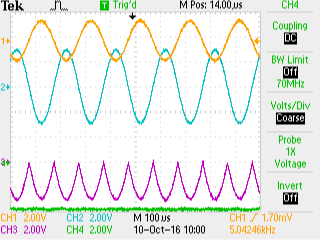
\includegraphics[width=0.8\textwidth]{./img/scisniete.png}
					\caption{\small{Ściśnięty czujnik}}
				\end{figure} \noindent
				\begin{figure}[H]
					\centering
					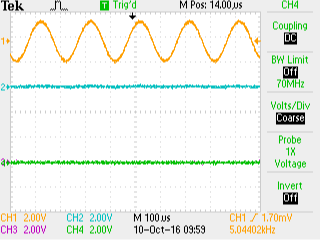
\includegraphics[width=0.8\textwidth]{./img/punkt_neutralny.png}
					\caption{\small{Zero konstrukcyjne}}
				\end{figure} \noindent
				\begin{figure}[H]
					\centering
					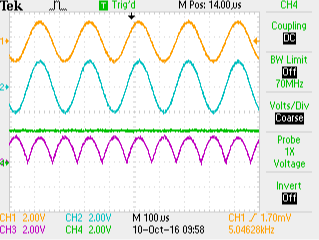
\includegraphics[width=0.8\textwidth]{./img/rozciagniete.png}
					\caption{\small{Ściśnięty czujnik}}
				\end{figure} \noindent
		\subsection{Wyznaczenie charakterystyki statycznej wzmacniacza pomiarowego z modulacją AM}
			\begin{figure}[H]
				\centering
				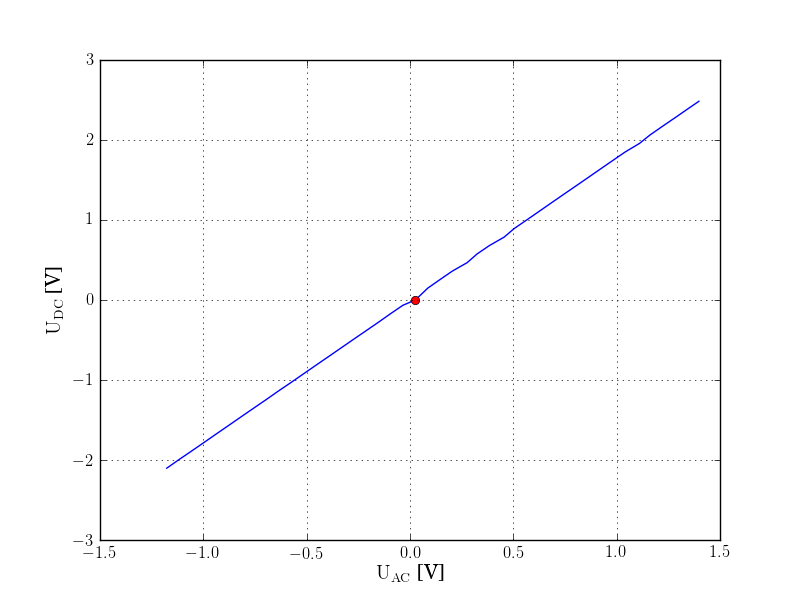
\includegraphics[width=0.8\textwidth]{./img/Uac_od_Udc.png}
				\caption{\small{Zależność }}
			\end{figure} \noindent
			\begin{figure}[H]
				\centering
				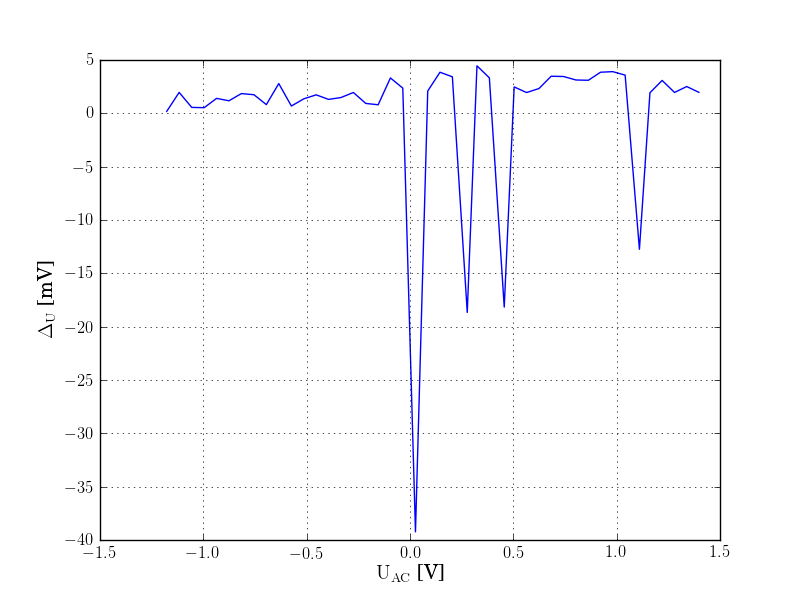
\includegraphics[width=0.8\textwidth]{./img/Uac_Udc_blad.png}
				\caption{\small{Ściśnięty czujnik}}
			\end{figure} \noindent
		\subsection{Wyznaczenie charakterystyki statycznej układu czujnik + tor z modulacją amplitudową}
			\begin{figure}[H]
				\centering
				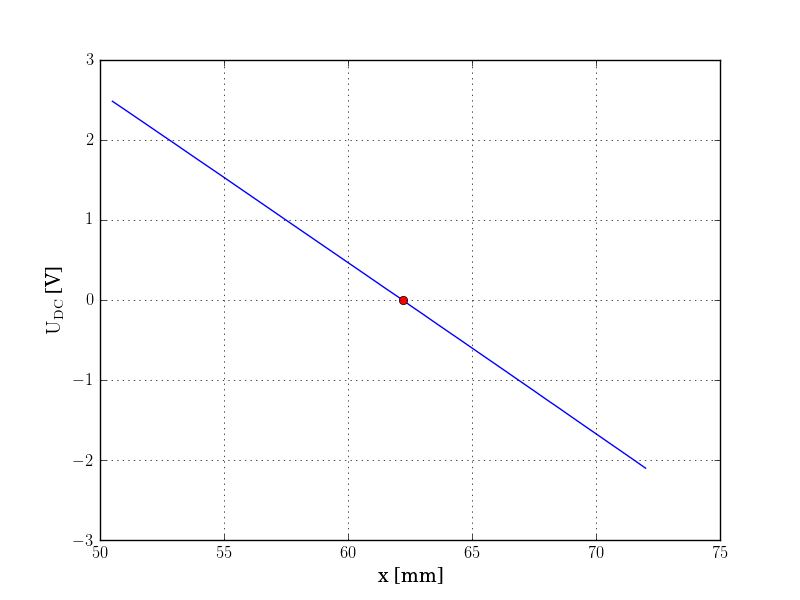
\includegraphics[width=0.8\textwidth]{./img/Udc_od_x.png}
				\caption{\small{Zależność }}
			\end{figure} \noindent
			\begin{figure}[H]
				\centering
				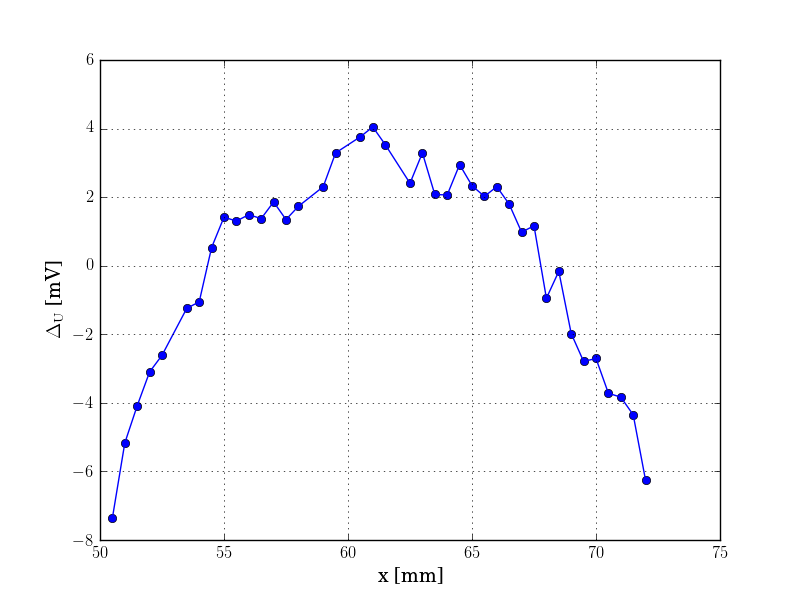
\includegraphics[width=0.8\textwidth]{./img/Udc_blad.png}
				\caption{\small{Ściśnięty czujnik}}
			\end{figure} \noindent
	\section{Wnioski i podsumowanie}
		Na podstawie ćwiczenia dowiedzieliśmy się dlaczego w zadanym torze pomiarowym wybrano konkretne wartości do przetwarzania informacji o przesunięciu rdzenia w czujniku. Z punktu drugiego dowiedzieliśmy się jak można zasymulować obecność czujnika przy pomocy zwykłego dzielnika napięcia.
		\newline \newline
		Obróbka dostępnych danych pokazuje w jakim zakresie badany czujnik zachowuje się liniowo i jak dobre jest przybliżenie przy pomocy prostej w przypadku odpowiednich charakterystyk. Ze względu na to, że błędy te są niewielkie w stosunku do wartości mierzonych można przyjąć, że linia prosta jest bardzo dobrym przybliżeniem charakterystyk i jako taka może być używana w modelach matematycznych.
		\newline \newline
		W przypadku likwidacji offsetu jaki towarzyszy pomiarom wartości można by było nawet założyć liniowość charakterystyki, co jest niezmiernie przydatne w wielu przypadkach.
\end{document}